\documentclass[10pt,twocolumn,letterpaper]{article}

\usepackage{dependable_dnn}
\usepackage{times}
\usepackage{epsfig}
\usepackage{graphicx}
\usepackage{amsmath}
\usepackage{amssymb}

\newcommand{\D}{\mathcal{D}}

% Include other packages here, before hyperref.

% If you comment hyperref and then uncomment it, you should delete
% egpaper.aux before re-running latex.  (Or just hit 'q' on the first latex
% run, let it finish, and you should be clear).
\usepackage[pagebackref=true,breaklinks=true,letterpaper=true,colorlinks,bookmarks=false]{hyperref}

\iccvfinalcopy % *** Uncomment this line for the final submission

\def\iccvPaperID{} % *** Enter the Paper ID here
\def\httilde{\mbox{\tt\raisebox{-.5ex}{\symbol{126}}}}

% Pages are numbered in submission mode, and unnumbered in camera-ready
\ificcvfinal\pagestyle{empty}\fi

\begin{document}

%%%%%%%%% TITLE - PLEASE UPDATE
\title{Boosting Self-Supervised Learning via Knowledge Transfer
	 \\ {\rm {\normalsize Seungmin Lee (profile2697@gmail.com; 2013-11420), Dept. of Computer Science and Engineering, Seoul National University}}} 

\maketitle
\thispagestyle{empty}

%%%%%%%%% BODY TEXT - ENTER YOUR RESPONSE BELOW

%%%%%%%%%%%%%%%%%
%%%%%%%%%%%%%%%%%
\section{Motivation}
\vspace{-0.2cm}
Self-supervised learning (SSL) aims to learn meaningful representations from pretext tasks for boosting the performance of target tasks. The pretext tasks do not require hand-made labels. Otherwise, the target tasks are typically assumed that the tasks do not have enough labels. Traditional SSL methods transfer the knowledge learned from the pretext task using fine-tuning. Despite using fine-tuning is a simple and effective way, the transfer methodology limits the design choices of network architectures since a pretext network and target network should have the same structure for the fine-tuning. In this setting, the architecture is limited to a simple structure because the target task does not have enough labels. For the same reason, the difficulty of the pretext task is also limited to an easy task because it should be solvable using the simple model. The proposed method tries to decouple the architectures of pretext tasks and target tasks using distillation.
 
\vspace{-0.3cm}
%%%%%%%%%%%%%%%%%
%%%%%%%%%%%%%%%%%
\section{Method}
\vspace{-0.2cm}
\subsection{Knowledge Transfer using Distillation}
\vspace{-0.2cm}
The proposed method uses distillation instead of fine-tuning for knowledge transfer. The distillation removes the coupling of the target task network architecture and pretext task network architecture. Additionally, the distillation also helps not to transfer specific knowledge of the pretext task like the weights of the fully-connected layers. The proposed knowledge transfer procedure consists of four steps: \textbf{(a)} train a pretext model on a pretext task. \textbf{(b)} extract cluster centroids of features from the pre-trained pretext model using the K-means algorithm. In this step, the features are generated using the images of the pretext tasks. \textbf{(c)} assign pseudo-labels to the target task images by finding the closest centroid of each image. Note a different dataset(like target dataset) than the one used in step (a) can be utilized in this step.\textbf{(d)} pre-train a task model using a classification problem of the pseudo-labels.
\vspace{-0.2cm}
\subsection{More Difficult Pretext Task: Jigsaw++}
\vspace{-0.2cm}
By decoupling the architectures of the pretext task and the target task, the proposed method can use a deeper pretext task model and thus more difficult but representative pretext tasks. This paper proposed a Jigsaw++ pretext task. This task is similar to the ordinary jigsaw puzzle, except it can contain some random tiles from other images. In this paper, the pretext task consists of 9 tiles, and at most, 2 tiles are from other images. The proposed task is harder than other pretext tasks, but it gives more characteristic features.
\vspace{-0.3cm}
\vspace{-0.3cm}
%%%%%%%%%%%%%%%%%
%%%%%%%%%%%%%%%%%
\section{Experiments and Analysis}
\vspace{-0.2cm}
There are many interesting experiments and analysis. In this section, I will briefly summarize the results.
\vspace{-0.3cm}
\paragraph{Impact of Cluster Centroids} 
The authors measured the performance by varying the number of centroids from 500 to 2000. They used the ImageNet dataset, so the optimal amount of the centroids is maybe about 1000. In these experiments, the performance increases as the number of centroids increases. However, the difference between the lowest and largest performance is marginal, which indicates the proposed method is pretty robust to the centroids number if the technique does not choose extremely a small amount.
\vspace{-0.3cm}
\paragraph{Comparison with Other SSL Methods}
The authors compared the proposed method to other SSL methods. According to the results, the pretext task model size seems pretty essential. The difference between distillation and fine-tuning using the same pretext task and the same model is marginal. However, using vgg as the pretext model instead of AlexNet boosts the performance, which indicates the decoupling the network structures is crucial.
\vspace{-0.3cm}
\paragraph{Classification with a Linear Classifier}
In this experiment, the authors compared the performances of linear classifiers trained on features from an arbitrary layer. Compared to other SSL methods, the proposed method seems to encode more characteristic features. The difference between the performances of the conv1 and conv4 is quite significant. This difference shows the choice of the intermediate layer used for transferring knowledge is crucial. Therefore, if we can find the optimal layer, it would be helpful to transfer adequate knowledge.
\vspace{-0.3cm}
\paragraph{Visualization}
The visualization also shows interesting results (Figure.~\ref{fig:vis}). The images that lie around the same cluster centroid share similar characteristics.

 \begin{figure}[b]
	\centering
	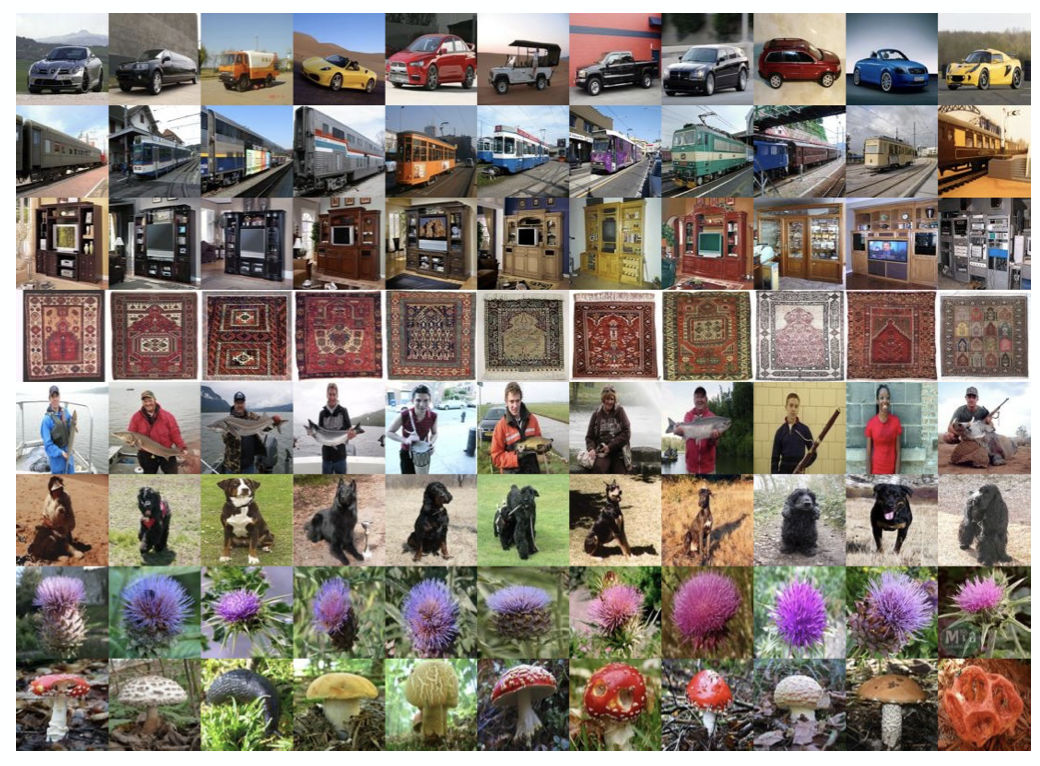
\includegraphics[height=4cm]{figures/vis.png}
	\caption{Each rows are the images that lie around the same centroid.}\label{fig:vis}
\end{figure}

{\small
\bibliographystyle{ieee}
%\bibliography{egbib}
}

\end{document}
